\chapter{Phân tích khảo sát hệ thống bộ nhớ}
\label{ch:memory_analysis}

\section{Nguyễn Trường Thái}

\subsection{Khảo sát cấu hình máy}
Khảo sát cấu hình của máy và hệ thống bộ nhớ của máy đang sử dụng (Bộ nhớ trong: ROM, RAM, Cache System,..) được thực hiện bằng phần mềm CPU-Z.



\subsubsection{CPU}
\begin{figure}[H]
    \centering
    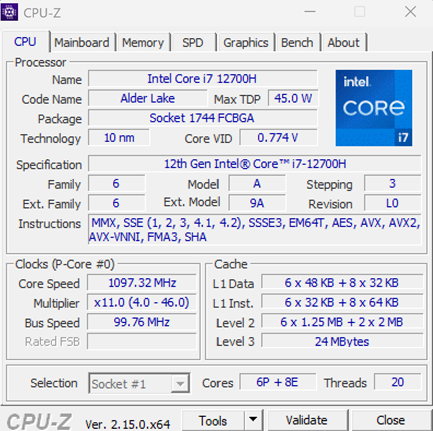
\includegraphics[width=0.8\textwidth]{Thái/Picture12.png}
    \caption{Intel Core i7-12700H – 14 Nhân – 20 Luồng}
\end{figure}


\subsubsection{Cache}
\begin{figure}[H]
    \centering
    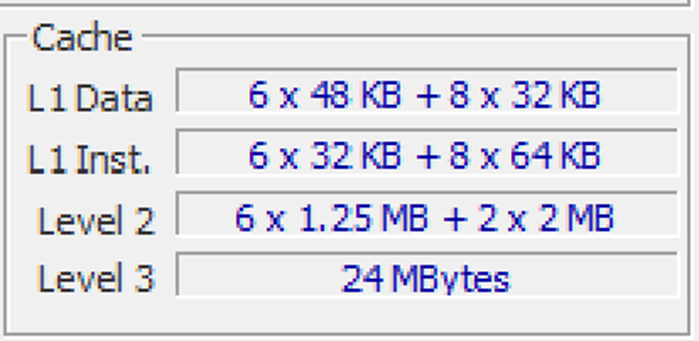
\includegraphics[width=0.8\textwidth]{Thái/Picture13.png}
    \caption{Hệ thống cache của máy tính bao gồm các cấp L1, L2, và L3.}
\end{figure}


\subsubsection{RAM}
\begin{figure}[H]
    \centering
    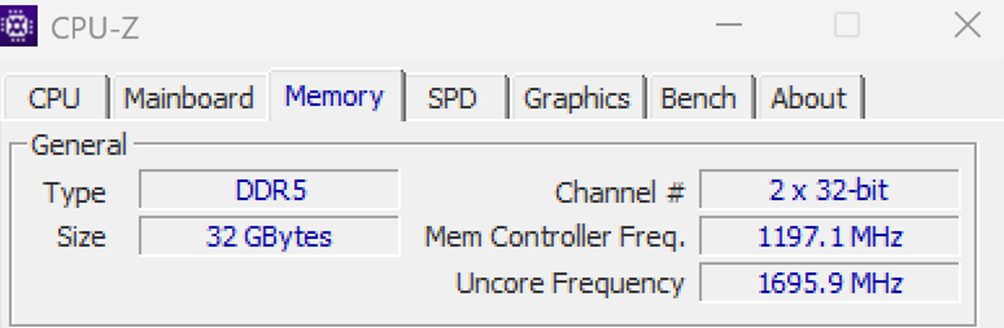
\includegraphics[width=0.8\textwidth]{Thái/Picture14.png}
    \caption{32Gb.}
\end{figure}

\subsubsection{Bộ nhớ ngoài}
\begin{figure}[H]
    \centering
    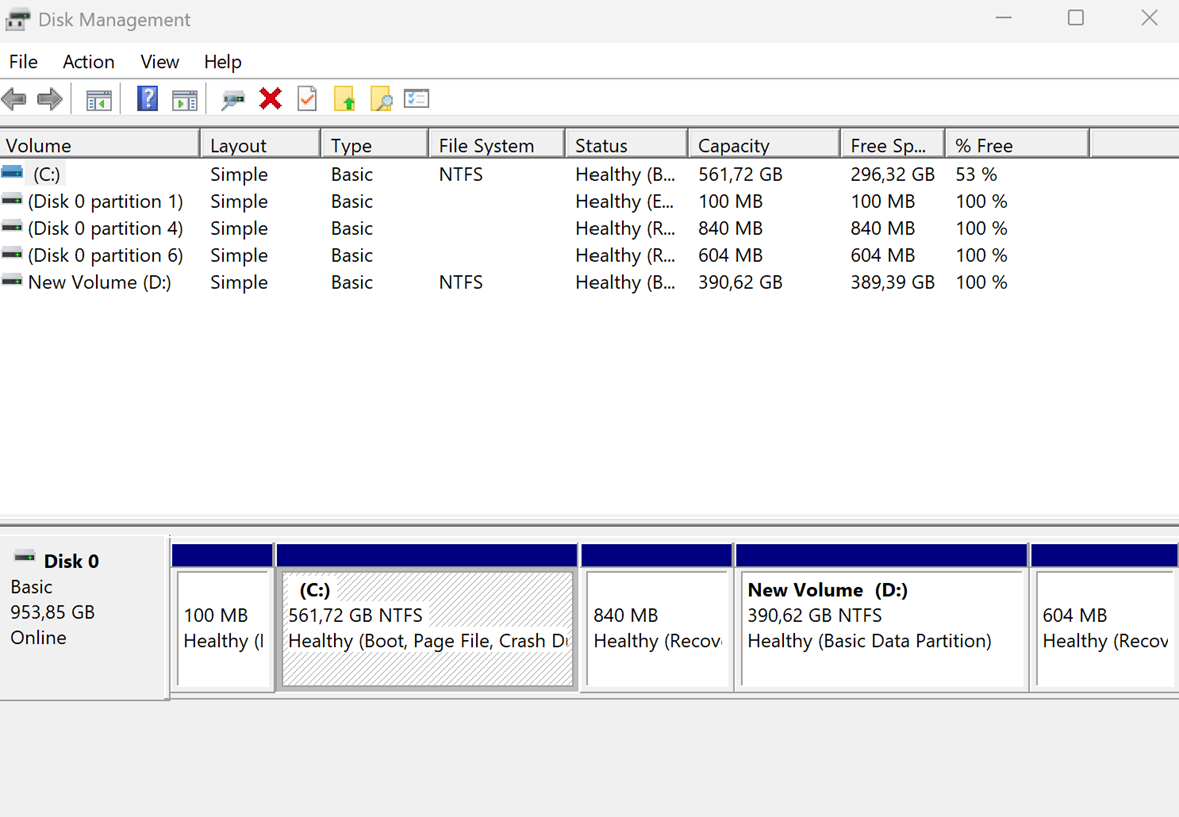
\includegraphics[width=0.9\textwidth]{Thái/Picture15.png}
\end{figure}


\subsubsection{Các thiết bị vào ra}
\begin{figure}[H]
    \centering
     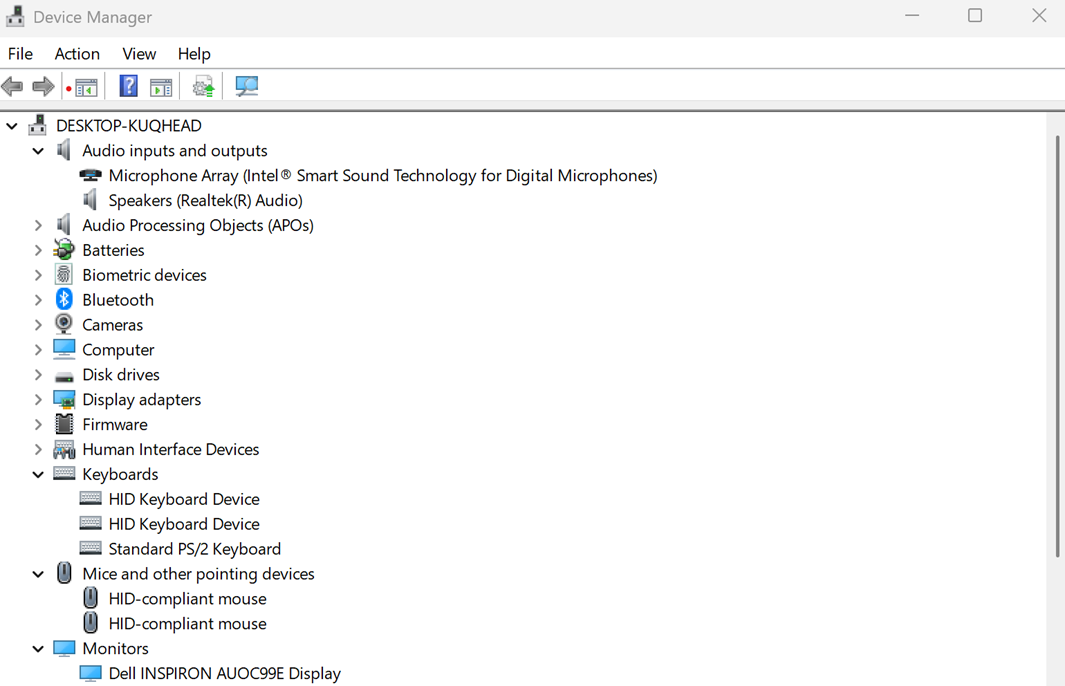
\includegraphics[width=1\textwidth]{Thái/Picture16.png}
     \caption{ Bao gồm bàn phím, chuột, màn hình, và các cổng kết nối.}
\end{figure}




\subsection{Khảo sát nội dung các thanh ghi}


\subsubsection{Giải thích nội dung các thanh ghi}
Dùng công cụ Debug khảo sát nội dung các thanh ghi IP, DS, ES, SS, CS, BP, SP

\begin{itemize}
    \item Công cụ sử dụng: emu8086 microprocessor emulator
    \item Các bước thực hiện:
    \item Mở file .asm bằng phần mềm trên
    \item Chọn emulate trên thanh công cụ rồi chọn nút debug nằm cuối của cửa sổ vừa mở ra
    \item Chạy Single step để xem kết quả debug từng mã lệnh từ đầu đến cuối
\end{itemize}

\begin{figure}[H]
    \centering
    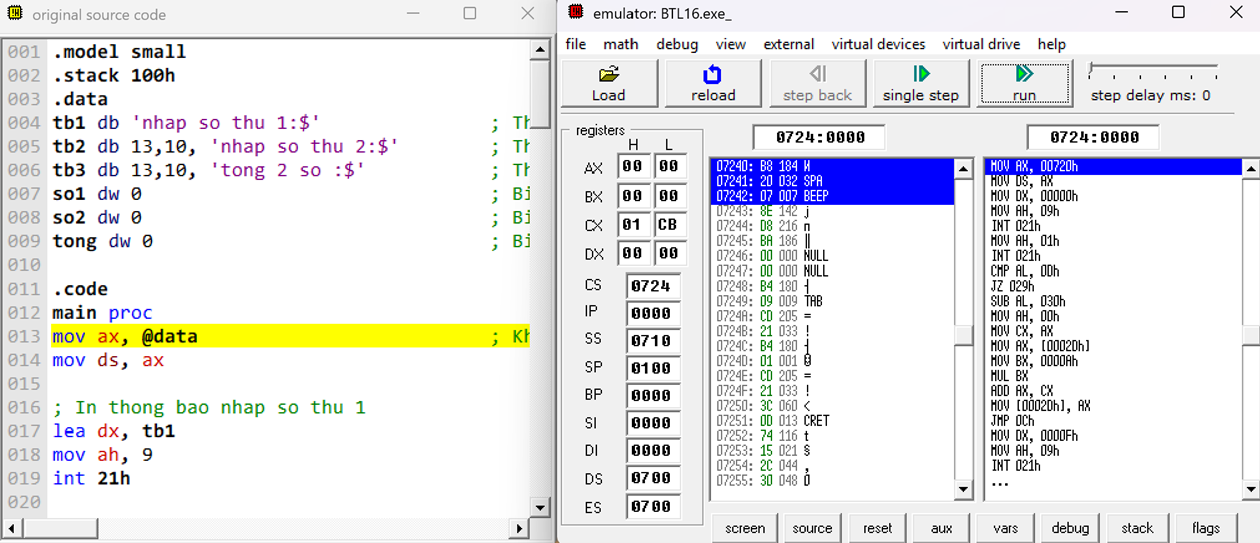
\includegraphics[width=1\textwidth]{Thái/Picture17.png}
\end{figure}

\begin{figure}[H]
    \centering
    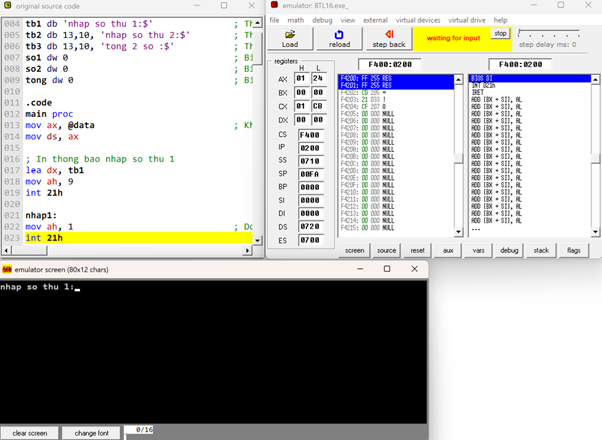
\includegraphics[width=1\textwidth]{Thái/Picture18.png}
\end{figure}

\begin{figure}[H]
    \centering
    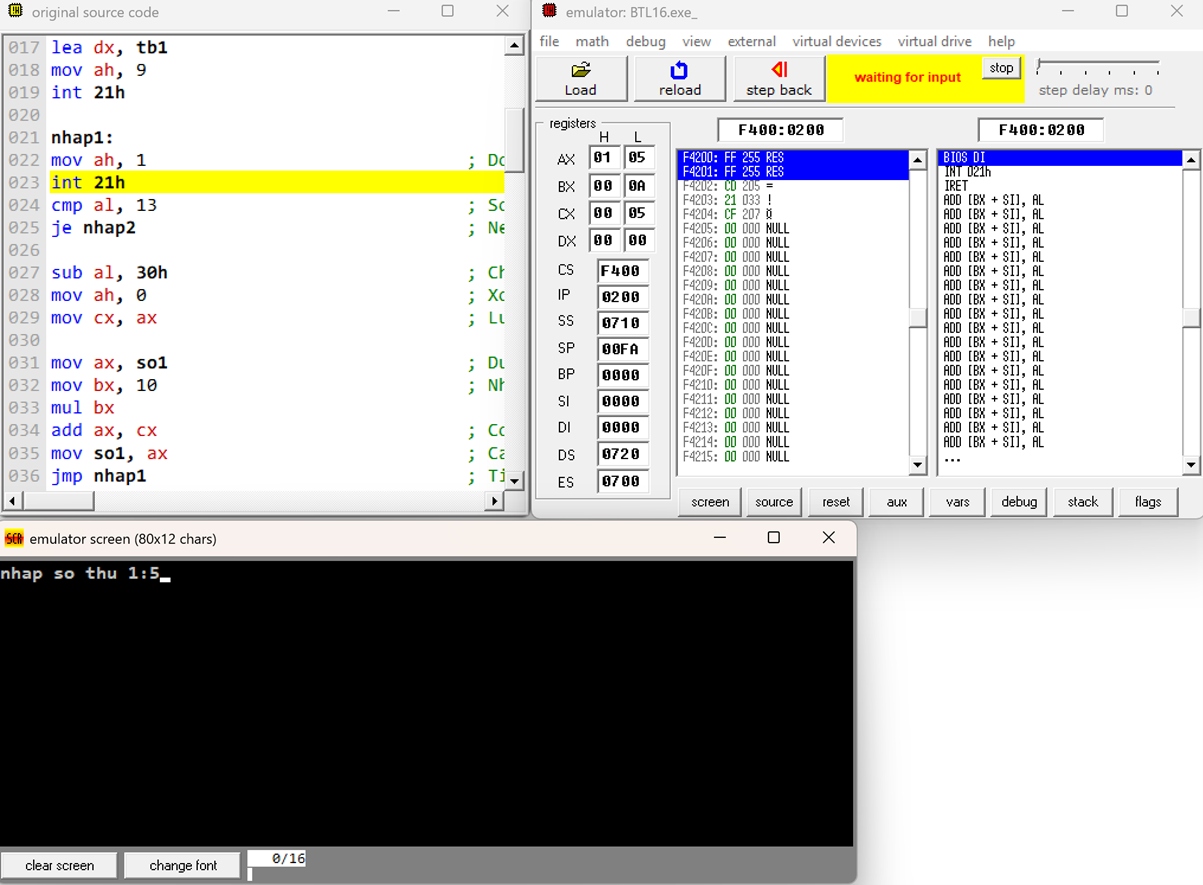
\includegraphics[width=0.95\textwidth]{Thái/Picture19.png}
\end{figure}

\begin{figure}[H]
    \centering
    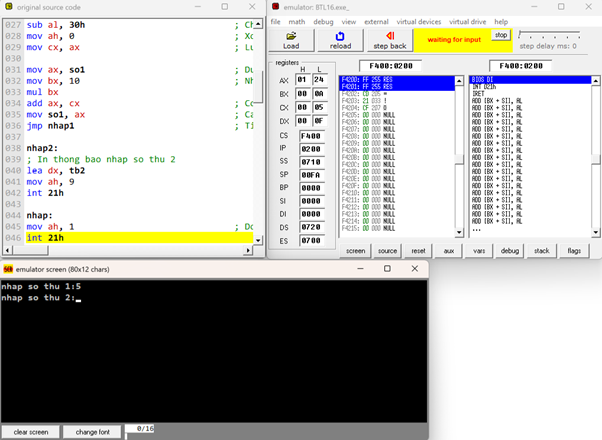
\includegraphics[width=0.95\textwidth]{Thái/Picture20.png}
\end{figure}

\begin{figure}[H]
    \centering
    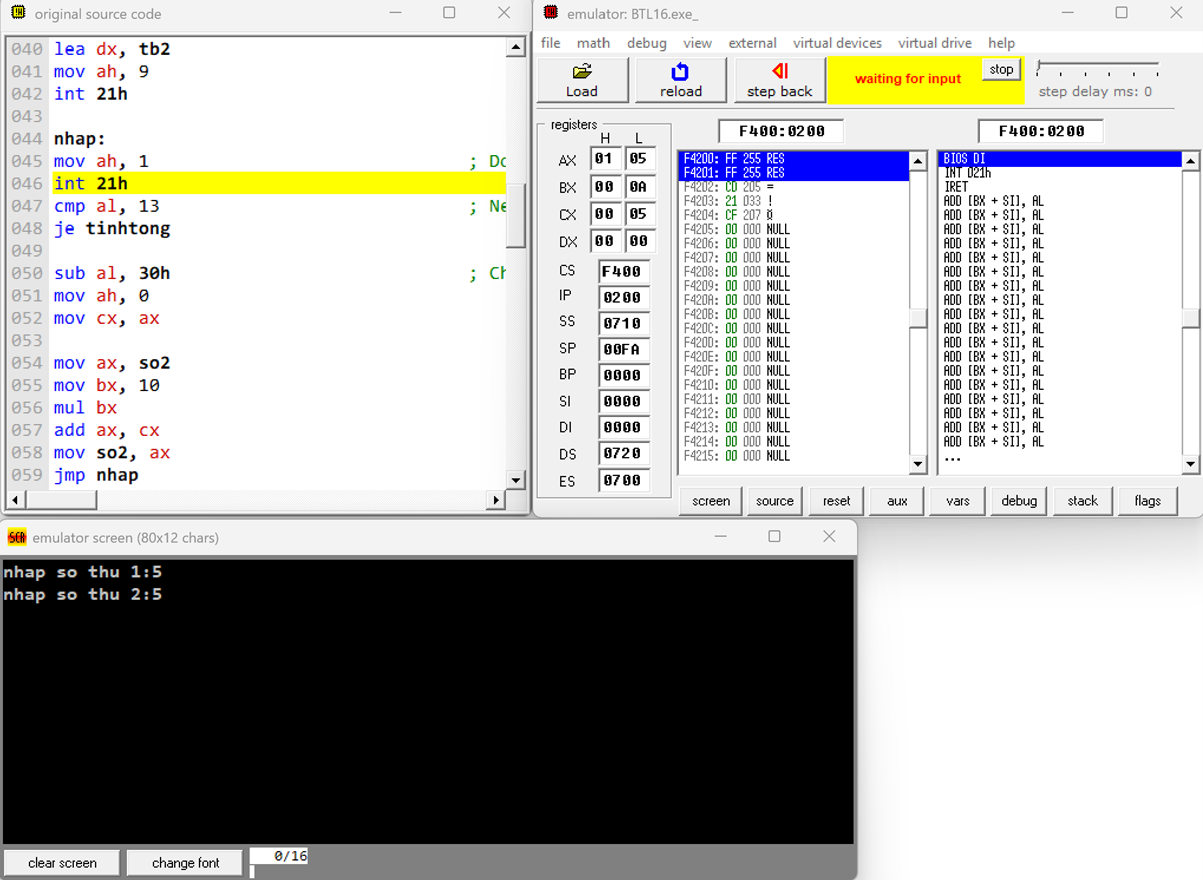
\includegraphics[width=0.95\textwidth]{Thái/Picture21.png}
\end{figure}

\begin{figure}[H]
    \centering
    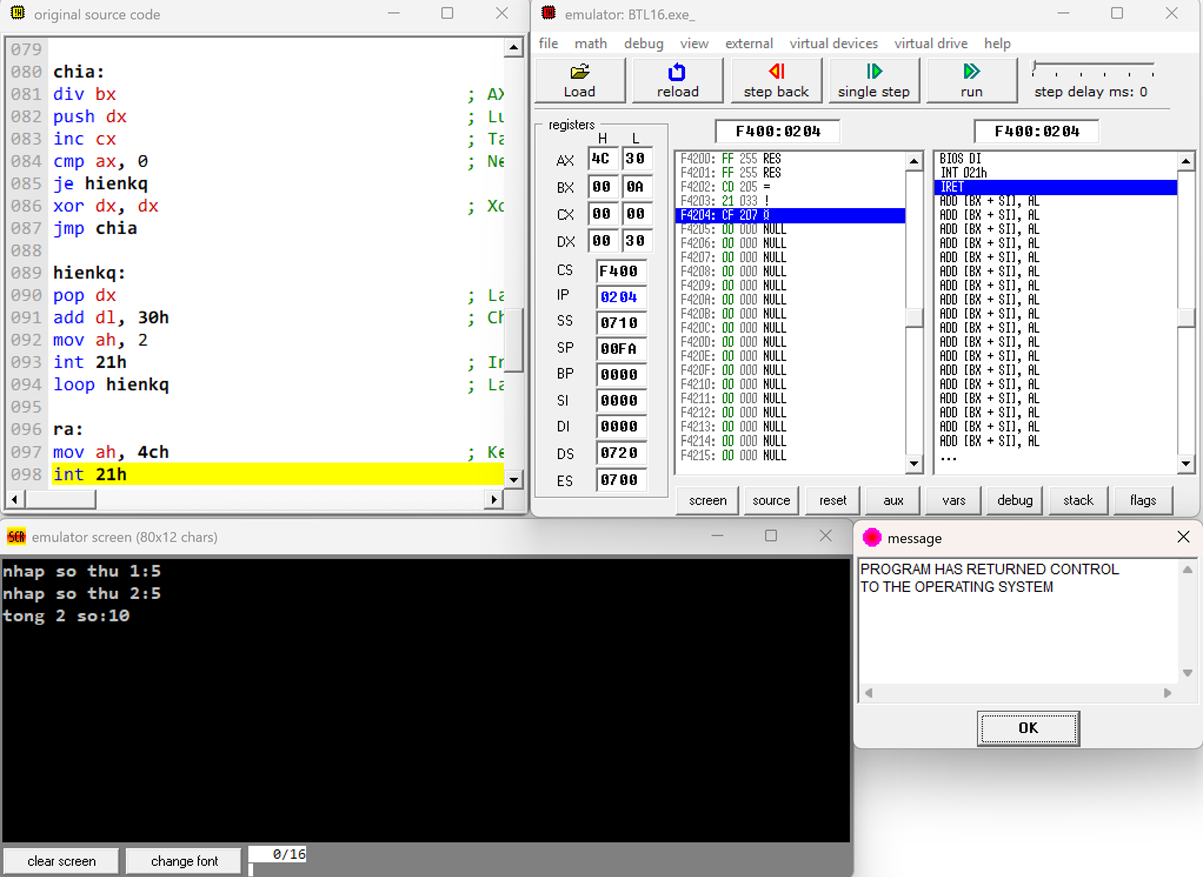
\includegraphics[width=0.95\textwidth]{Thái/Picture22.png}
\end{figure}


\subsection{Giải thích nội dung các thanh ghi}
Khi chương trình bắt đầu chạy, hệ điều hành tự động khởi tạo các thanh ghi, vùng nhớ và cấp phát không gian địa chỉ cho chương trình. Tương ứng với các câu lệnh trong mã nguồn, nội dung các thanh ghi có thể thay đổi hoặc không.

\subsubsection{IP (Instruction Pointer)}
\begin{itemize}
    \item IP là thanh ghi trỏ đến địa chỉ của lệnh tiếp theo sẽ được thực thi trong mã máy.
    \item Khi một chương trình được thực thi, IP được cập nhật để trỏ đến lệnh tiếp theo trong mã nguồn. Điều này giúp CPU biết lệnh nào sẽ được thực thi tiếp theo.
\end{itemize}

\subsubsection{DS (Data Segment) và SI (Source Index)}
\begin{itemize}
    \item DS là thanh ghi chỉ đến phân đoạn dữ liệu, nơi dữ liệu chương trình được lưu trữ.
    \item SI thường được sử dụng trong các phép toán dữ liệu và là một trong các thanh ghi chỉ địa chỉ.
    \item Khi chương trình yêu cầu truy cập dữ liệu từ bộ nhớ, DS và SI thường được sử dụng để xác định vị trí của dữ liệu trong bộ nhớ.
\end{itemize}

\subsubsection{SS (Stack Segment) và BP (Base Pointer)}
\begin{itemize}
    \item SS là thanh ghi chỉ đến phân đoạn ngăn xếp (stack segment), nơi các giá trị cục bộ và địa chỉ của các hàm được lưu trữ.
    \item BP thường được sử dụng để trỏ đến địa chỉ cơ sở của ngăn xếp (base of stack).
    \item Ngăn xếp được sử dụng để lưu trữ các giá trị trung gian và địa chỉ trả về từ các hàm con (subroutines) trong quá trình thực thi chương trình.
\end{itemize}

\subsubsection{SP (Stack Pointer)}
\begin{itemize}
    \item SP là thanh ghi chỉ đến đỉnh của ngăn xếp (top of stack).
    \item Khi dữ liệu được đẩy (push) hoặc rút (pop) ra khỏi ngăn xếp, SP sẽ thay đổi để chỉ đến vị trí mới nhất trong ngăn xếp.
    \item SP cũng được sử dụng để cấp phát không gian mới cho dữ liệu trong ngăn xếp.
\end{itemize}

\subsection{Cơ chế quản lý bộ nhớ}

Cụ thể, trong trường hợp của đoạn chương trình chuyển xâu ký tự thành xâu in hoa và in thường tương ứng, ta có cơ chế quản lý bộ nhớ như sau:

\subsubsection{Khởi tạo bộ nhớ}
\begin{itemize}
    \item Khi chương trình bắt đầu, HĐH sẽ cấp phát các đoạn mã (code), dữ liệu (data), và ngăn xếp (stack) cho chương trình.
    \item Đoạn mã chứa các lệnh chương trình, đoạn dữ liệu chứa các biến, và đoạn ngăn xếp dùng để lưu trữ dữ liệu tạm thời.
\end{itemize}

\subsubsection{Phân đoạn bộ nhớ}
\begin{itemize}
    \item CS (Code Segment) trỏ tới đoạn mã của chương trình.
    \item DS (Data Segment) trỏ tới đoạn dữ liệu của chương trình.
    \item SS (Stack Segment) trỏ tới đoạn ngăn xếp của chương trình.
\end{itemize}

\subsubsection{Quản lý ngăn xếp}
\begin{itemize}
    \item Ngăn xếp được sử dụng để lưu trữ tạm thời dữ liệu và địa chỉ trả về khi gọi hàm.
    \item SP được khởi tạo với giá trị từ khai báo .Stack 100H, nghĩa là kích thước ngăn xếp là 256 byte.
\end{itemize}



\subsubsection{Diễn giải mã nguồn và ảnh hưởng đến thanh ghi}
\begin{itemize}
    \item \textbf{Khởi tạo đoạn dữ liệu:} 
\begin{figure}[H]
    \centering
    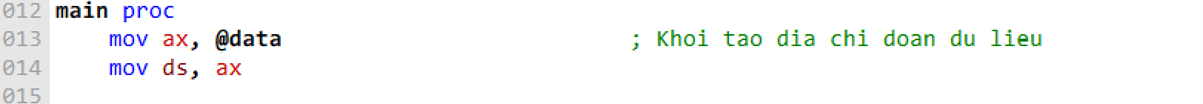
\includegraphics[width=1\textwidth]{Thái/Picture23.png}
\end{figure}
    DS trỏ tới đoạn dữ liệu. Thanh ghi AX được dùng làm trung gian để nạp địa chỉ đoạn dữ liệu vào DS.
    
    \item \textbf{Hiển thị thông báo và đọc chuỗi ký tự:} 
\begin{figure}[H]
    \centering
    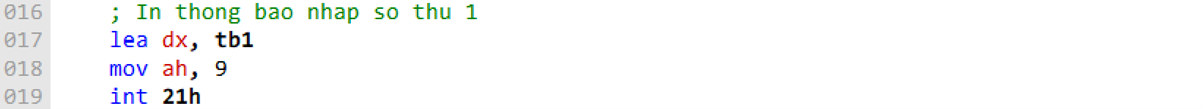
\includegraphics[width=1\textwidth]{Thái/Picture24.png}
\end{figure}
    AH = 9 gọi hàm in chuỗi của ngắt 21h; DX chứa địa chỉ chuỗi cần in.

    \item \textbf{Nhập số thứ nhất từng chữ số và ghép thành số nguyên:} 
\begin{figure}[H]
    \centering
    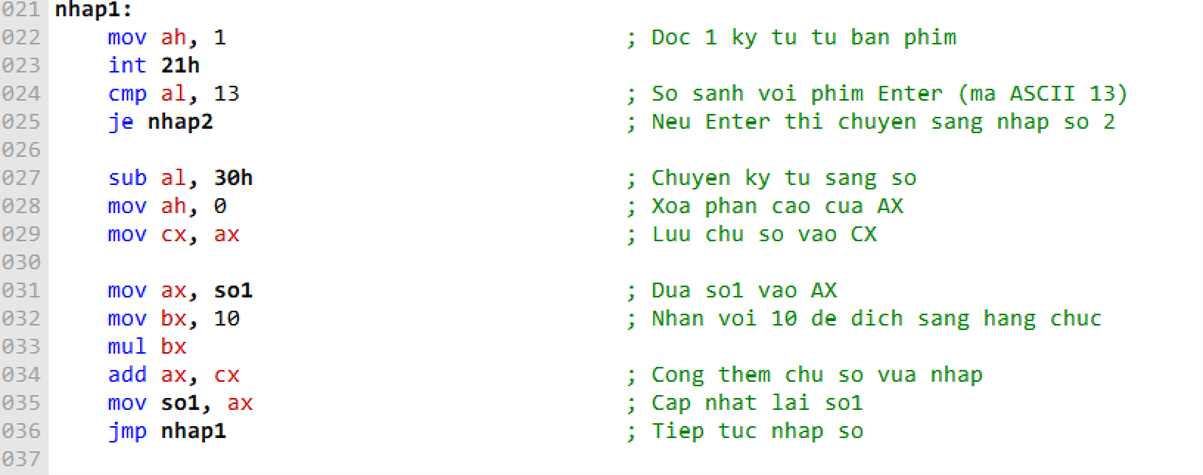
\includegraphics[width=1\textwidth]{Thái/Picture25.png}
\end{figure}    
    AH = 1 để đọc từng ký tự. Nếu AL = 13 (Enter), nhảy sang nhãn \texttt{nhap2}. Ký tự nhập được chuyển từ ASCII sang số, sau đó: \\
    so1 = so1 × 10 + chữ số mới.

    \item \textbf{Hiển thị thông báo nhập số thứ hai và nhập tương tự:} 
\begin{figure}[H]
    \centering
    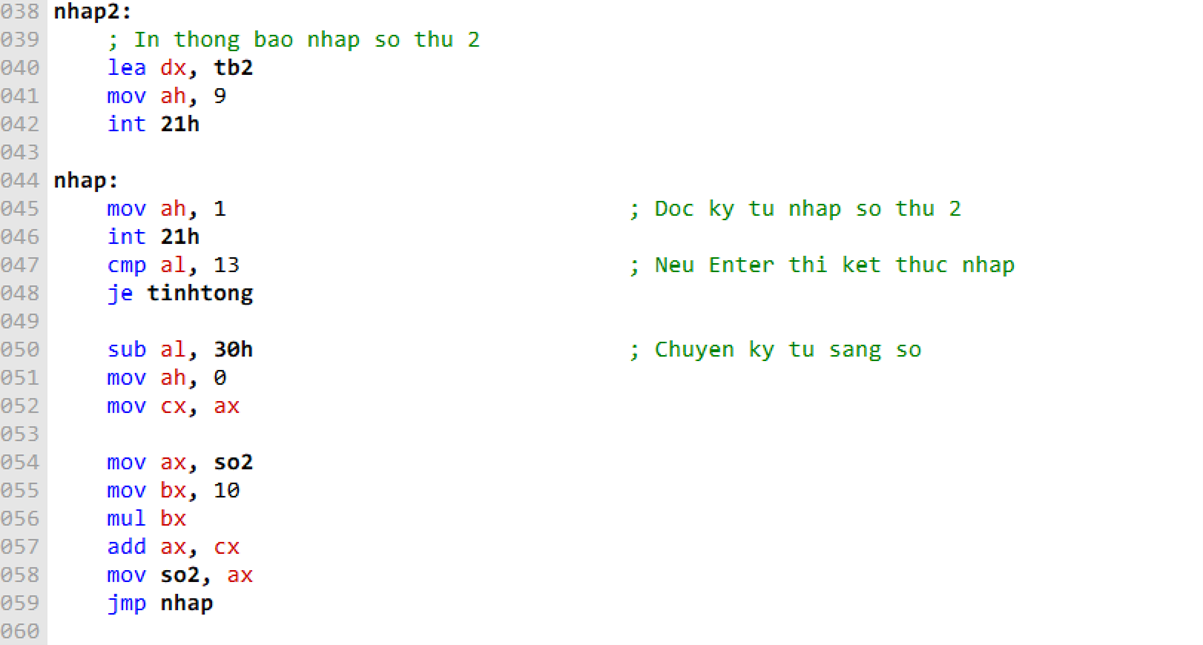
\includegraphics[width=1\textwidth]{Thái/Picture26.png}
\end{figure}
    In chuỗi thông báo với AH = 9, sau đó đọc từng ký tự bằng AH = 1. Nếu nhấn Enter thì nhảy đến nhãn \texttt{tinhtong}. \\
    so2 = so2 × 10 + chữ số mới (tương tự như so1).

\item \textbf{Tính tổng hai số, tách chữ số và in kết quả:}
\begin{figure}[H]
    \centering
    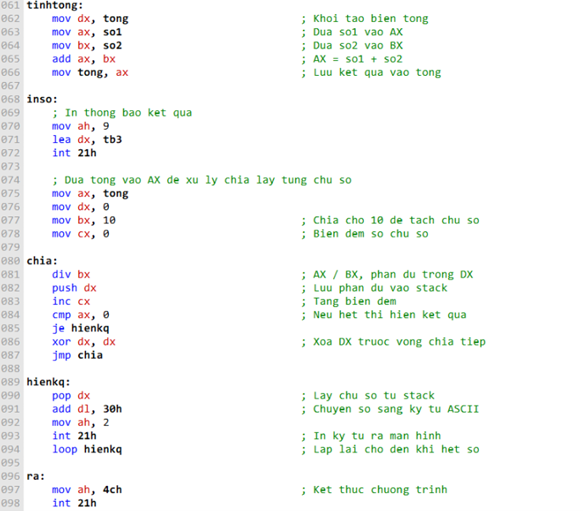
\includegraphics[width=1\textwidth]{Thái/Picture27.png}
\end{figure}
         Tính tổng: 
        \texttt{MOV AX, so1}, \texttt{MOV BX, so2}, \texttt{ADD AX, BX}, \texttt{MOV tong, AX} 
        
         In thông báo: 
        \texttt{MOV AH,9}, \texttt{LEA DX, tb3}, \texttt{INT 21h} 
        
        Chuẩn bị chia tách chữ số: 
        \texttt{MOV AX, tong}, \texttt{MOV DX,0}, \texttt{MOV BX,10}, \texttt{MOV CX,0} 
        
         \textbf{Vòng lặp chia (chia lấy chữ số, lưu stack):}
        \begin{itemize}
            \item \texttt{DIV BX}: Chia AX cho 10 → dư (chữ số) vào DX
            \item \texttt{PUSH DX}: Lưu chữ số lên stack (đảo ngược)
            \item \texttt{INC CX}: Tăng đếm chữ số
            \item \texttt{CMP AX,0 + JE hienkq}: Nếu AX=0 thì sang vòng in kết quả
            \item \texttt{XOR DX,DX}, \texttt{JMP chia}: Xóa DX và tiếp tục vòng chia
        \end{itemize}
        
         \textbf{Vòng lặp hienkq (lấy và in chữ số):}
        \begin{itemize}
            \item \texttt{POP DX}, \texttt{ADD DL,30h}: Lấy số và chuyển sang ASCII
            \item \texttt{MOV AH,2}, \texttt{INT 21h}: In ra màn hình
            \item \texttt{LOOP hienkq}: Lặp lại đến khi CX = 0
        \end{itemize}

         \textbf{Kết thúc chương trình:} \\
        \texttt{MOV AH,4Ch}, \texttt{INT 21h}
    
    
\end{itemize}


\section{Vũ Quang Huy}

\subsection{Khảo sát cấu hình máy}
Khảo sát cấu hình của máy và hệ thống bộ nhớ của máy đang sử dụng (Bộ nhớ trong: ROM, RAM, Cache System,..) được thực hiện bằng phần mềm CPU-Z.

\subsubsection{CPU}
\begin{figure}[H]
    \centering
    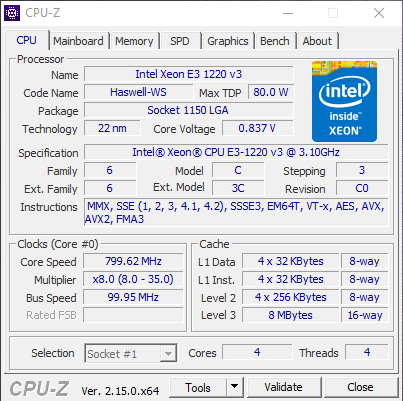
\includegraphics[width=0.9\textwidth]{Huy/2.1.1.png}
    \caption{Intel Xeon E3 1220 v3 - 4 Nhân - 4 Luồng.}
\end{figure}

\subsubsection{Cache}
\begin{figure}[H]
    \centering
    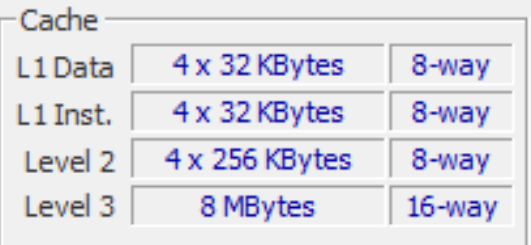
\includegraphics[width=0.9\textwidth]{Huy/2.1.2.png}
    \caption{Hệ thống cache của máy tính bao gồm các cấp L1, L2, và L3.}
\end{figure}

\subsubsection{RAM}
\begin{figure}[H]
    \centering
    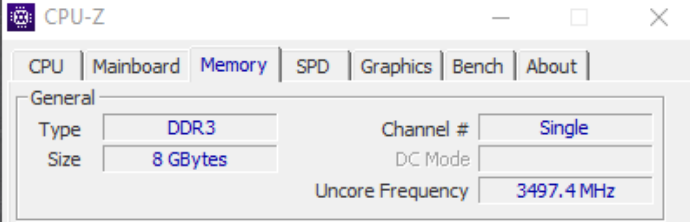
\includegraphics[width=0.9\textwidth]{Huy/2.1.3.png}
    \caption{8Gb.}
\end{figure}


\subsubsection{Bộ nhớ ngoài}
\begin{figure}[H]
    \centering
    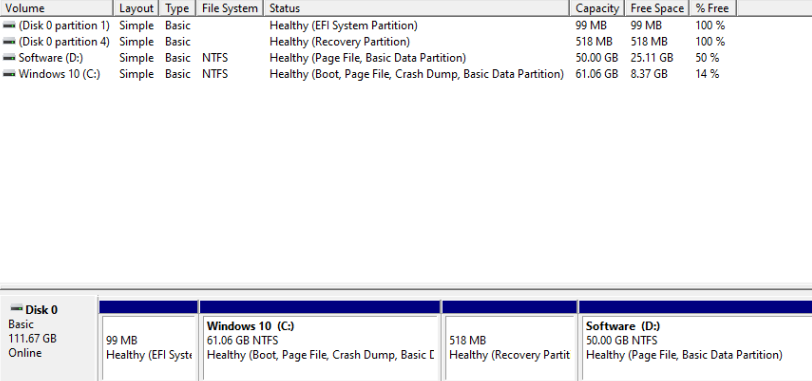
\includegraphics[width=1\textwidth]{Huy/2.1.4.png}
\end{figure}


\subsubsection{Các thiết bị vào ra}
\begin{figure}[H]
    \centering
    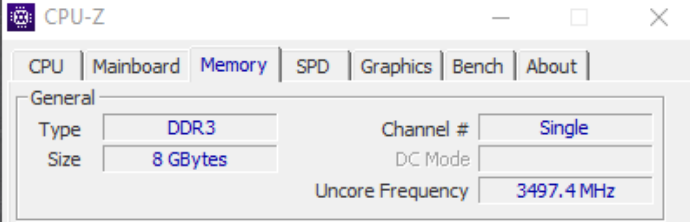
\includegraphics[width=0.9\textwidth]{Huy/2.1.3.png}
    \caption{Bao gồm bàn phím, chuột, màn hình, và các cổng kết nối.}
\end{figure}


\subsection{Khảo sát nội dung các thanh ghi}


\subsubsection{Giải thích nội dung các thanh ghi}
Dùng công cụ Debug khảo sát nội dung các thanh ghi IP, DS, ES, SS, CS, BP, SP

\begin{itemize}
    \item Công cụ sử dụng: emu8086 microprocessor emulator
    \item Các bước thực hiện:
    \item Mở file .asm bằng phần mềm trên
    \item Chọn emulate trên thanh công cụ rồi chọn nút debug nằm cuối của cửa sổ vừa mở ra
    \item Chạy Single step để xem kết quả debug từng mã lệnh từ đầu đến cuối
\end{itemize}

\begin{figure}[H]
    \centering
    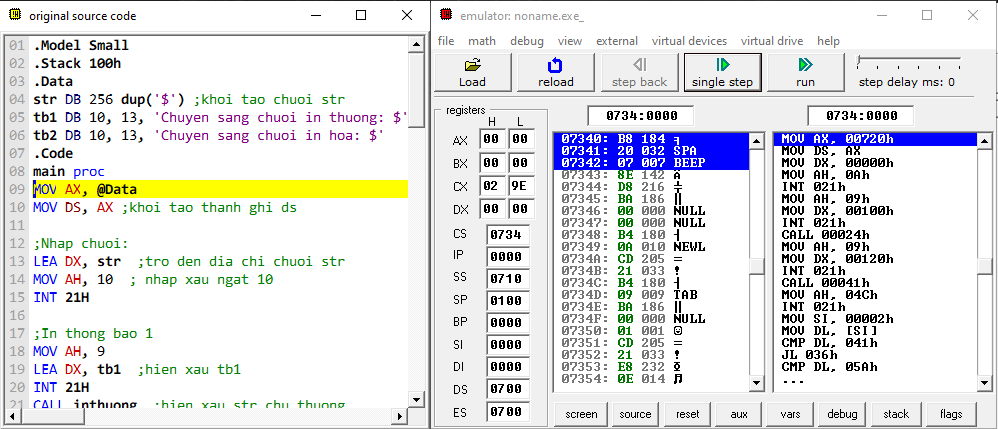
\includegraphics[width=1\textwidth]{Huy/2.2.1.png}
\end{figure}

\begin{figure}[H]
    \centering
    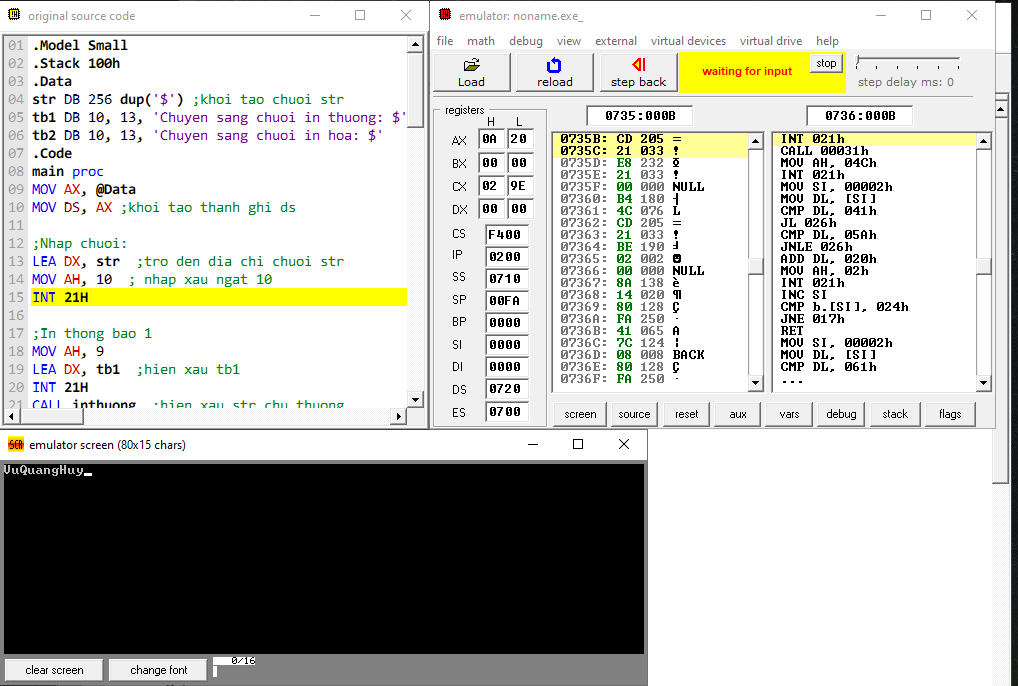
\includegraphics[width=1\textwidth]{Huy/2.2.2.png}
\end{figure}

\begin{figure}[H]
    \centering
    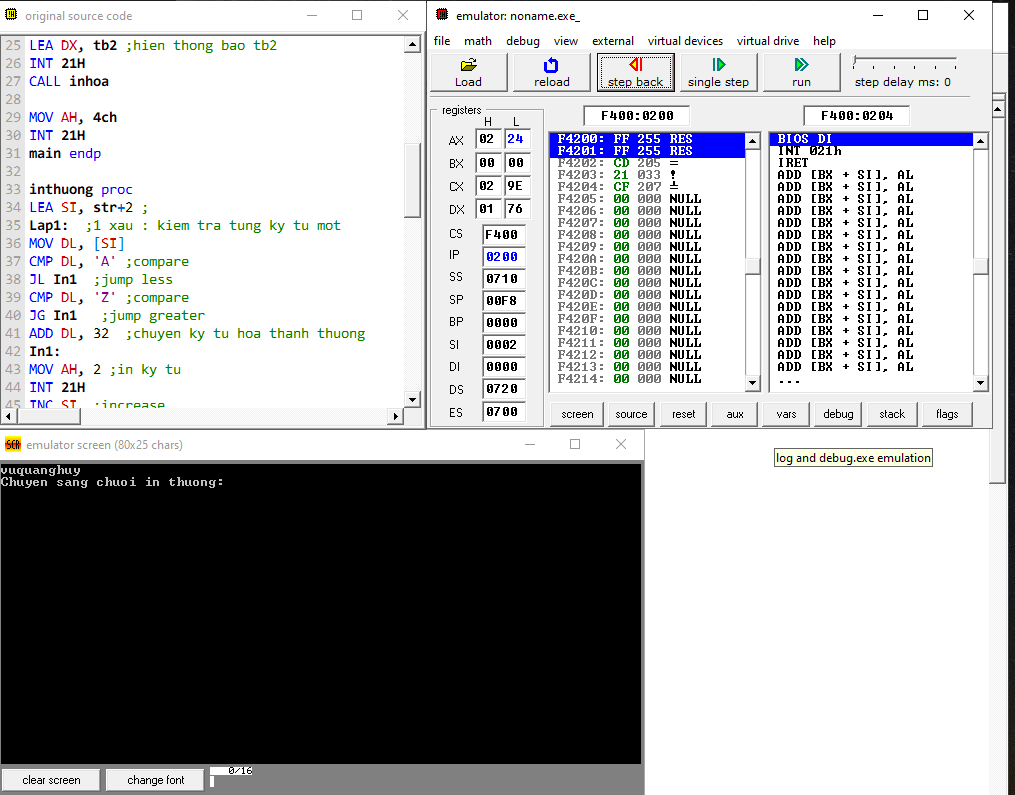
\includegraphics[width=0.9\textwidth]{Huy/2.2.3.png}
\end{figure}

\begin{figure}[H]
    \centering
    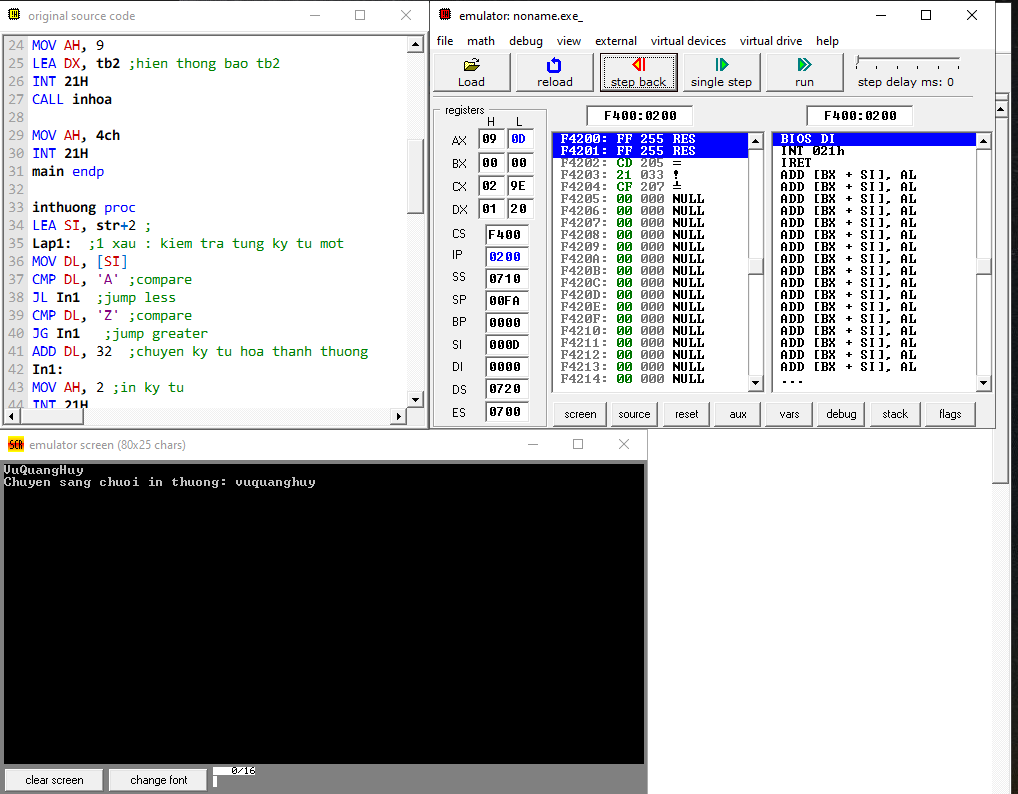
\includegraphics[width=0.9\textwidth]{Huy/2.2.4.png}
\end{figure}

\begin{figure}[H]
    \centering
    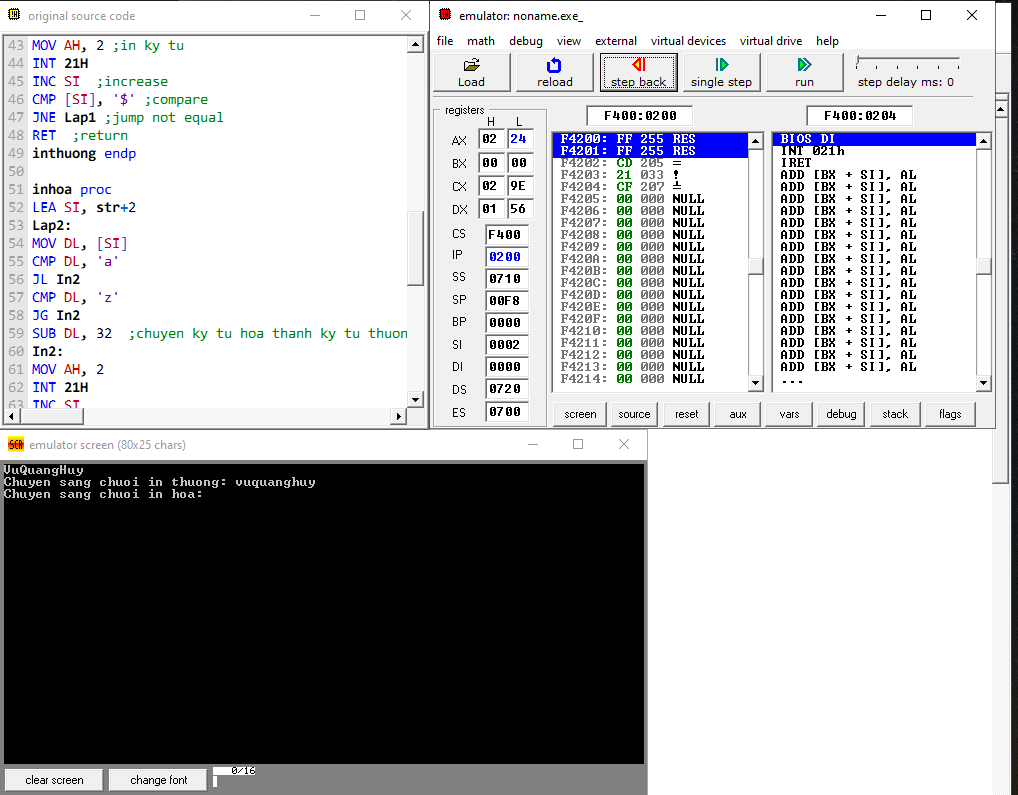
\includegraphics[width=0.9\textwidth]{Huy/2.2.5.png}
\end{figure}

\begin{figure}[H]
    \centering
    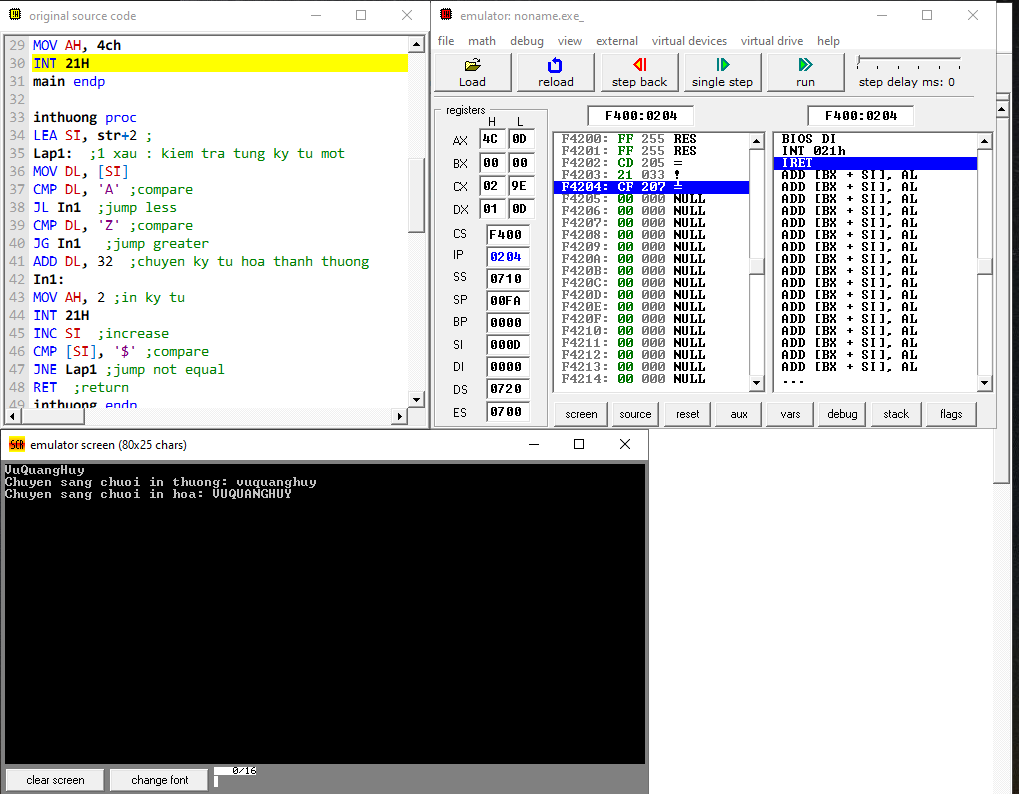
\includegraphics[width=0.9\textwidth]{Huy/2.2.6.png}
\end{figure}

\subsection{Giải thích nội dung các thanh ghi}
Khi chương trình bắt đầu chạy, hệ điều hành tự động khởi tạo các thanh ghi, vùng nhớ và cấp phát không gian địa chỉ cho chương trình. Tương ứng với các câu lệnh trong mã nguồn, nội dung các thanh ghi có thể thay đổi hoặc không.

\subsubsection{IP (Instruction Pointer)}
\begin{itemize}
    \item IP là thanh ghi trỏ đến địa chỉ của lệnh tiếp theo sẽ được thực thi trong mã máy.
    \item Khi một chương trình được thực thi, IP được cập nhật để trỏ đến lệnh tiếp theo trong mã nguồn. Điều này giúp CPU biết lệnh nào sẽ được thực thi tiếp theo.
\end{itemize}

\subsubsection{DS (Data Segment) và SI (Source Index)}
\begin{itemize}
    \item DS là thanh ghi chỉ đến phân đoạn dữ liệu, nơi dữ liệu chương trình được lưu trữ.
    \item SI thường được sử dụng trong các phép toán dữ liệu và là một trong các thanh ghi chỉ địa chỉ.
    \item Khi chương trình yêu cầu truy cập dữ liệu từ bộ nhớ, DS và SI thường được sử dụng để xác định vị trí của dữ liệu trong bộ nhớ.
\end{itemize}

\subsubsection{SS (Stack Segment) và BP (Base Pointer)}
\begin{itemize}
    \item SS là thanh ghi chỉ đến phân đoạn ngăn xếp (stack segment), nơi các giá trị cục bộ và địa chỉ của các hàm được lưu trữ.
    \item BP thường được sử dụng để trỏ đến địa chỉ cơ sở của ngăn xếp (base of stack).
    \item Ngăn xếp được sử dụng để lưu trữ các giá trị trung gian và địa chỉ trả về từ các hàm con (subroutines) trong quá trình thực thi chương trình.
\end{itemize}

\subsubsection{SP (Stack Pointer)}
\begin{itemize}
    \item SP là thanh ghi chỉ đến đỉnh của ngăn xếp (top of stack).
    \item Khi dữ liệu được đẩy (push) hoặc rút (pop) ra khỏi ngăn xếp, SP sẽ thay đổi để chỉ đến vị trí mới nhất trong ngăn xếp.
    \item SP cũng được sử dụng để cấp phát không gian mới cho dữ liệu trong ngăn xếp.
\end{itemize}

\subsection{Cơ chế quản lý bộ nhớ}

Cụ thể, trong trường hợp của đoạn chương trình chuyển xâu ký tự thành xâu in hoa và in thường tương ứng, ta có cơ chế quản lý bộ nhớ như sau:

\subsubsection{Khởi tạo bộ nhớ}
\begin{itemize}
    \item Khi chương trình bắt đầu, HĐH sẽ cấp phát các đoạn mã (code), dữ liệu (data), và ngăn xếp (stack) cho chương trình.
    \item Đoạn mã chứa các lệnh chương trình, đoạn dữ liệu chứa các biến, và đoạn ngăn xếp dùng để lưu trữ dữ liệu tạm thời.
\end{itemize}

\subsubsection{Phân đoạn bộ nhớ}
\begin{itemize}
    \item CS (Code Segment) trỏ tới đoạn mã của chương trình.
    \item DS (Data Segment) trỏ tới đoạn dữ liệu của chương trình.
    \item SS (Stack Segment) trỏ tới đoạn ngăn xếp của chương trình.
\end{itemize}

\subsubsection{Quản lý ngăn xếp}
\begin{itemize}
    \item Ngăn xếp được sử dụng để lưu trữ tạm thời dữ liệu và địa chỉ trả về khi gọi hàm.
    \item SP được khởi tạo với giá trị từ khai báo .Stack 100H, nghĩa là kích thước ngăn xếp là 256 byte.
\end{itemize}


\section{Lê Huy Hải}

\subsection{Khảo sát cấu hình máy}
Khảo sát cấu hình của máy và hệ thống bộ nhớ của máy đang sử dụng (Bộ nhớ trong: ROM, RAM, Cache System,..) được thực hiện bằng phần mềm CPU-Z.

\subsubsection{CPU}
\begin{figure}[H]
    \centering
    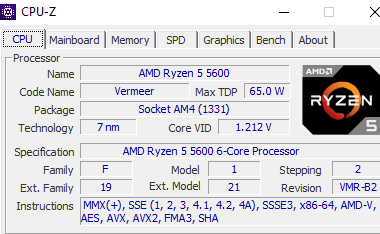
\includegraphics[width=0.8\textwidth]{Hải/Image_10.png}
    \caption{ADM-Ryzen 5-5600 – 6 nhân – 12 luồng.}
\end{figure}

\subsubsection{Cache}
\begin{figure}[H]
    \centering
    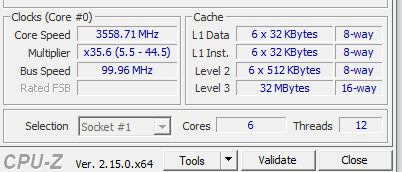
\includegraphics[width=0.9\textwidth]{Hải/Image_11.png}
    \caption{Hệ thống cache của máy tính bao gồm các cấp L1, L2, và L3.}
\end{figure}

\subsubsection{RAM}
\begin{figure}[H]
    \centering
    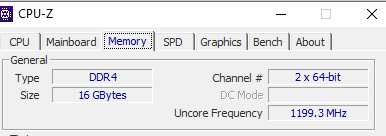
\includegraphics[width=0.9\textwidth]{Hải/Image_12.png}
    \caption{16Gb.}
\end{figure}

\subsubsection{Bộ nhớ ngoài}
\begin{figure}[H]
    \centering
    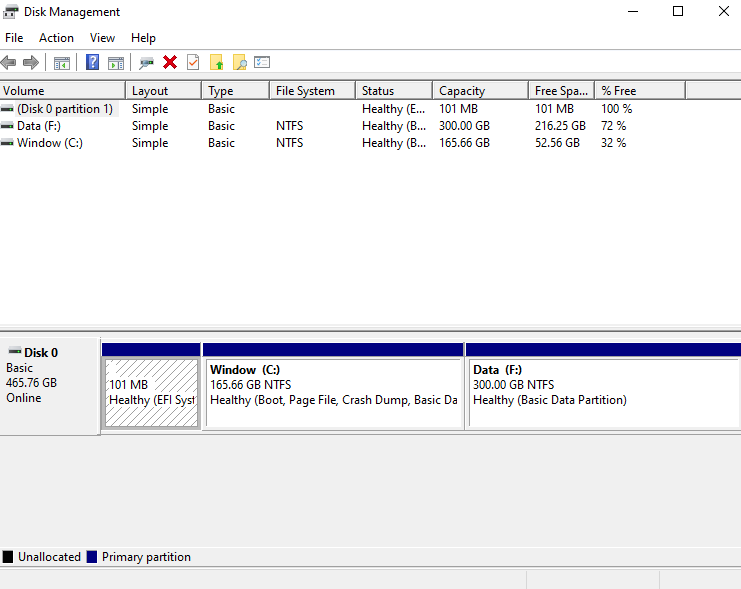
\includegraphics[width=0.9\textwidth]{Hải/Image_13.png}
\end{figure}

\subsubsection{Các thiết bị vào ra}
\begin{figure}[H]
    \centering
    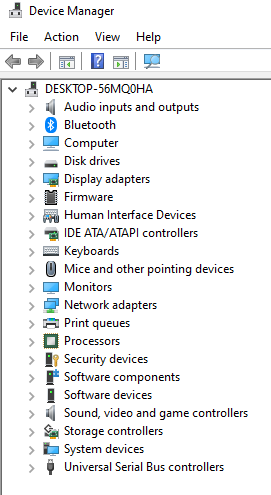
\includegraphics[width=0.7\textwidth]{Hải/Image_14.png}
    \caption{Các thiết bị vào ra bao gồm bàn phím, chuột, màn hình, và các cổng kết nối.}
\end{figure}


\subsection{Khảo sát nội dung các thanh ghi}


\subsubsection{Giải thích nội dung các thanh ghi}
Dùng công cụ Debug khảo sát nội dung các thanh ghi IP, DS, ES, SS, CS, BP, SP

\begin{itemize}
    \item Công cụ sử dụng: emu8086 microprocessor emulator
    \item Các bước thực hiện:
    \item Mở file .asm bằng phần mềm trên
    \item Chọn emulate trên thanh công cụ rồi chọn nút debug nằm cuối của cửa sổ vừa mở ra
    \item Chạy Single step để xem kết quả debug từng mã lệnh từ đầu đến cuối
\end{itemize}

\begin{figure}[H]
    \centering
    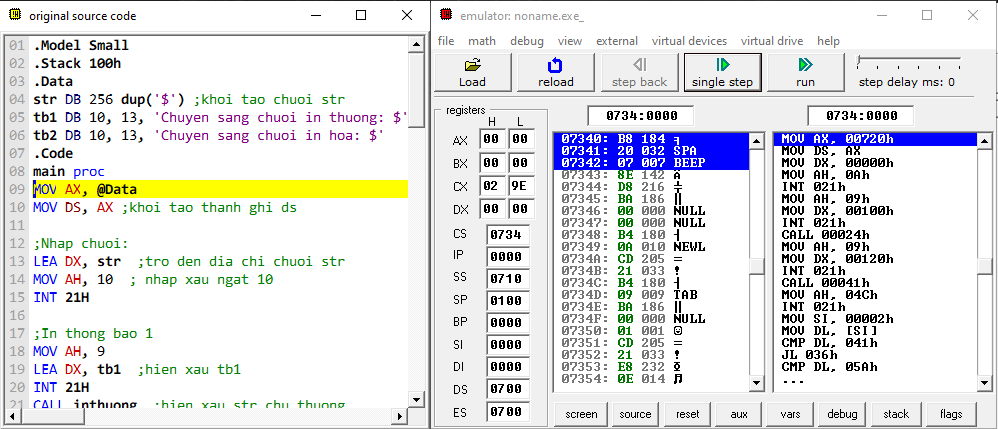
\includegraphics[width=1\textwidth]{Hải/Image_15.png}
\end{figure}

\begin{figure}[H]
    \centering
    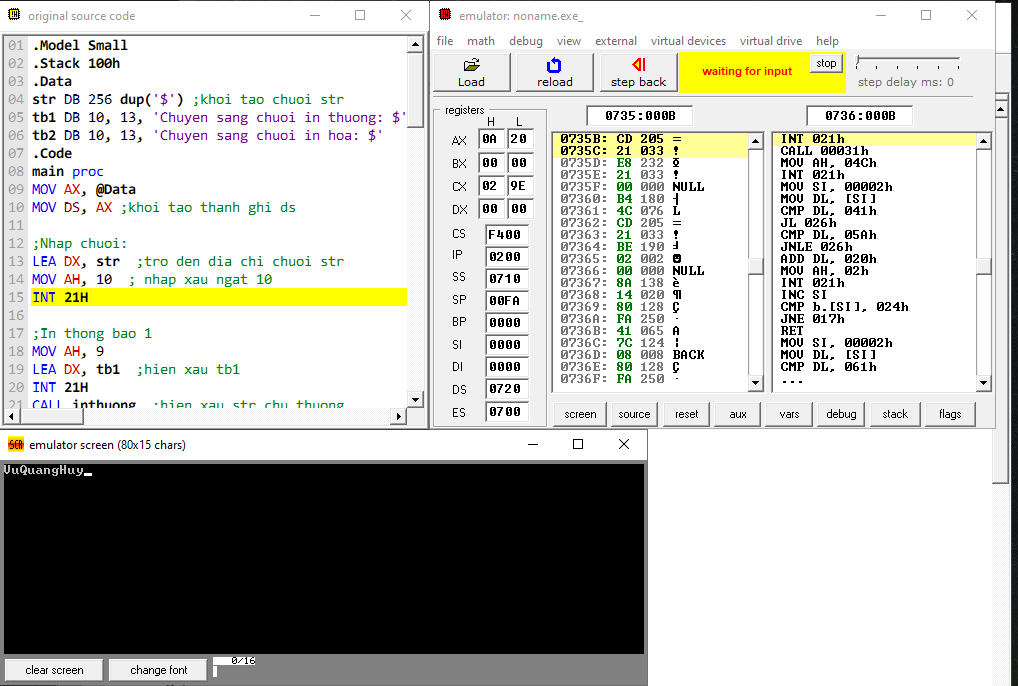
\includegraphics[width=0.95\textwidth]{Hải/Image_16.png}
\end{figure}

\begin{figure}[H]
    \centering
    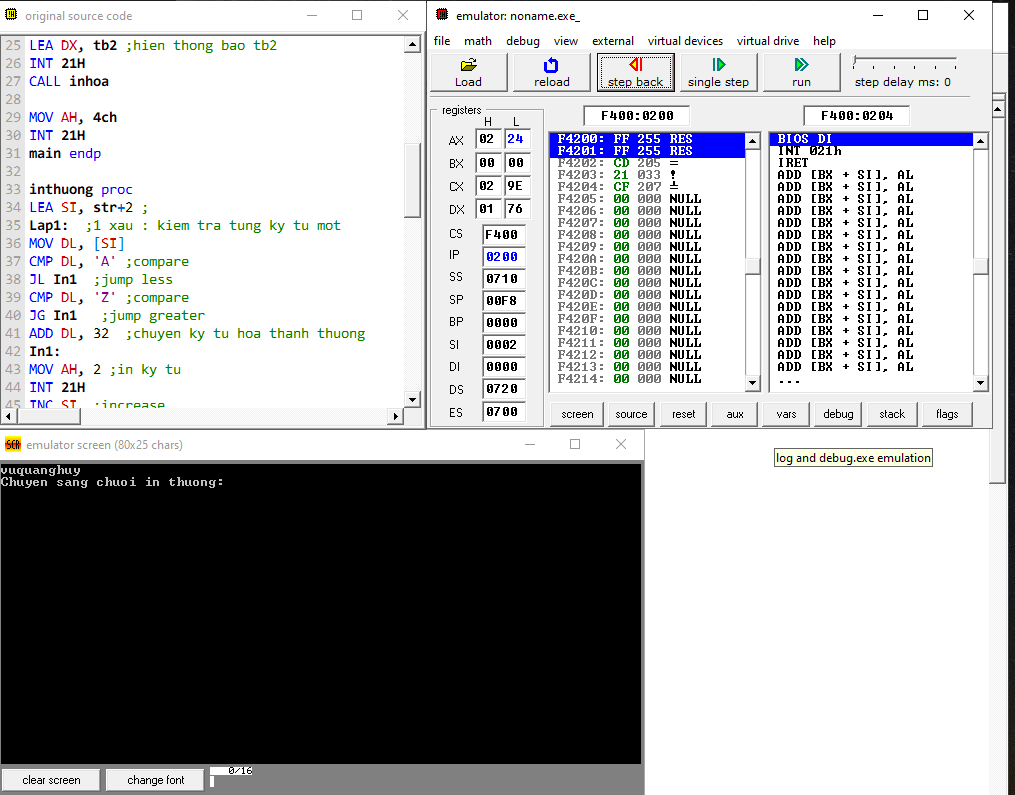
\includegraphics[width=0.95\textwidth]{Hải/Image_17.png}
\end{figure}

\begin{figure}[H]
    \centering
    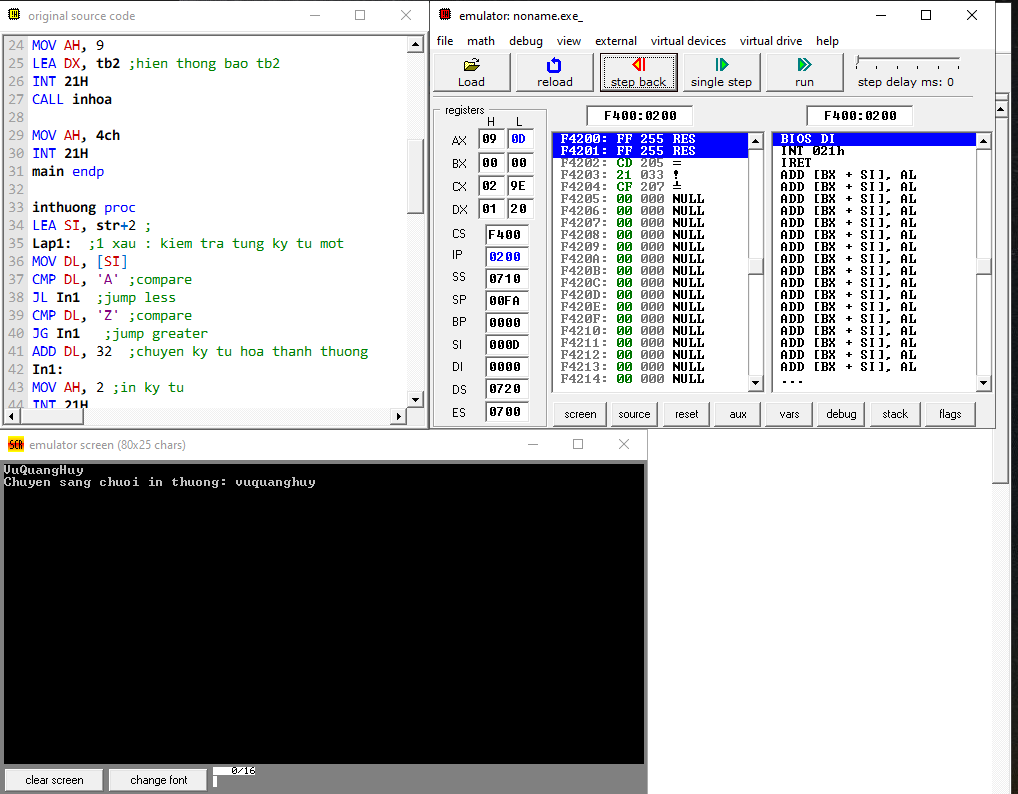
\includegraphics[width=0.9\textwidth]{Hải/Image_18.png}
\end{figure}

\begin{figure}[H]
    \centering
    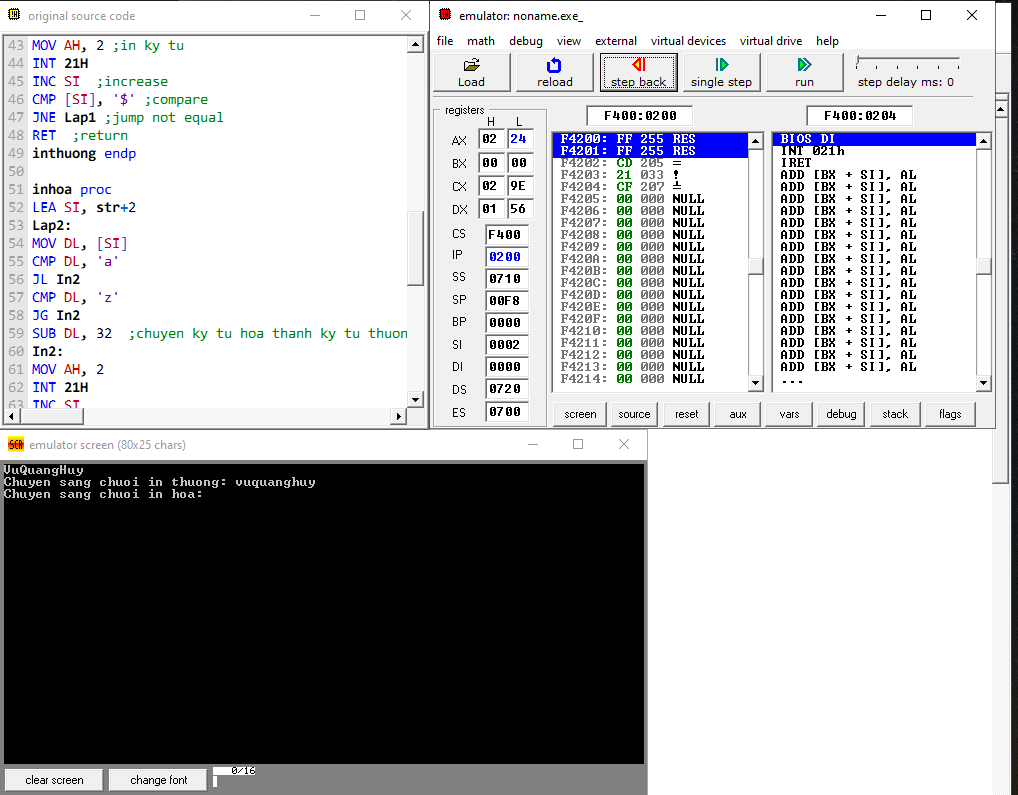
\includegraphics[width=0.9\textwidth]{Hải/Image_19.png}
\end{figure}

\begin{figure}[H]
    \centering
    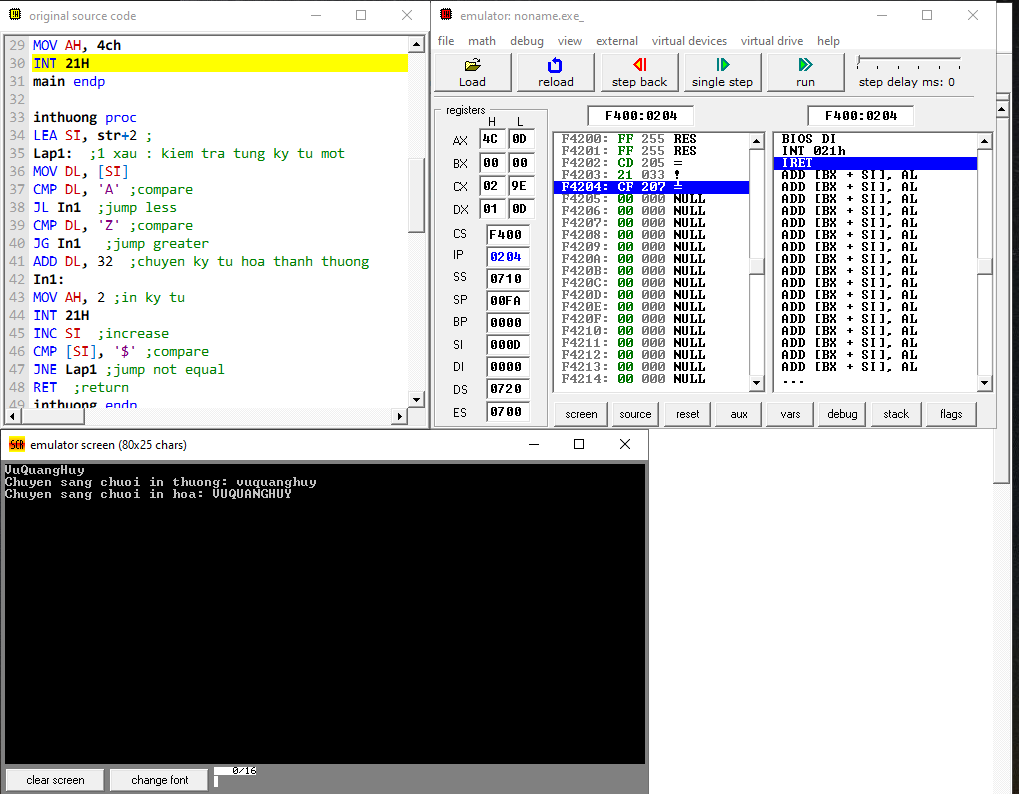
\includegraphics[width=1\textwidth]{Hải/Image_20.png}
\end{figure}


\subsection{Giải thích nội dung các thanh ghi}
Khi chương trình bắt đầu chạy, hệ điều hành tự động khởi tạo các thanh ghi, vùng nhớ và cấp phát không gian địa chỉ cho chương trình. Tương ứng với các câu lệnh trong mã nguồn, nội dung các thanh ghi có thể thay đổi hoặc không.

\subsubsection{IP (Instruction Pointer)}
\begin{itemize}
    \item IP là thanh ghi trỏ đến địa chỉ của lệnh tiếp theo sẽ được thực thi trong mã máy.
    \item Khi một chương trình được thực thi, IP được cập nhật để trỏ đến lệnh tiếp theo trong mã nguồn. Điều này giúp CPU biết lệnh nào sẽ được thực thi tiếp theo.
\end{itemize}

\subsubsection{DS (Data Segment) và SI (Source Index)}
\begin{itemize}
    \item DS là thanh ghi chỉ đến phân đoạn dữ liệu, nơi dữ liệu chương trình được lưu trữ.
    \item SI thường được sử dụng trong các phép toán dữ liệu và là một trong các thanh ghi chỉ địa chỉ.
    \item Khi chương trình yêu cầu truy cập dữ liệu từ bộ nhớ, DS và SI thường được sử dụng để xác định vị trí của dữ liệu trong bộ nhớ.
\end{itemize}

\subsubsection{SS (Stack Segment) và BP (Base Pointer)}
\begin{itemize}
    \item SS là thanh ghi chỉ đến phân đoạn ngăn xếp (stack segment), nơi các giá trị cục bộ và địa chỉ của các hàm được lưu trữ.
    \item BP thường được sử dụng để trỏ đến địa chỉ cơ sở của ngăn xếp (base of stack).
    \item Ngăn xếp được sử dụng để lưu trữ các giá trị trung gian và địa chỉ trả về từ các hàm con (subroutines) trong quá trình thực thi chương trình.
\end{itemize}

\subsubsection{SP (Stack Pointer)}
\begin{itemize}
    \item SP là thanh ghi chỉ đến đỉnh của ngăn xếp (top of stack).
    \item Khi dữ liệu được đẩy (push) hoặc rút (pop) ra khỏi ngăn xếp, SP sẽ thay đổi để chỉ đến vị trí mới nhất trong ngăn xếp.
    \item SP cũng được sử dụng để cấp phát không gian mới cho dữ liệu trong ngăn xếp.
\end{itemize}

\subsection{Cơ chế quản lý bộ nhớ}

Cụ thể, trong trường hợp của đoạn chương trình chuyển xâu ký tự thành xâu in hoa và in thường tương ứng, ta có cơ chế quản lý bộ nhớ như sau:

\subsubsection{Khởi tạo bộ nhớ}
\begin{itemize}
    \item Khi chương trình bắt đầu, HĐH sẽ cấp phát các đoạn mã (code), dữ liệu (data), và ngăn xếp (stack) cho chương trình.
    \item Đoạn mã chứa các lệnh chương trình, đoạn dữ liệu chứa các biến, và đoạn ngăn xếp dùng để lưu trữ dữ liệu tạm thời.
\end{itemize}

\subsubsection{Phân đoạn bộ nhớ}
\begin{itemize}
    \item CS (Code Segment) trỏ tới đoạn mã của chương trình.
    \item DS (Data Segment) trỏ tới đoạn dữ liệu của chương trình.
    \item SS (Stack Segment) trỏ tới đoạn ngăn xếp của chương trình.
\end{itemize}

\subsubsection{Quản lý ngăn xếp}
\begin{itemize}
    \item Ngăn xếp được sử dụng để lưu trữ tạm thời dữ liệu và địa chỉ trả về khi gọi hàm.
    \item SP được khởi tạo với giá trị từ khai báo .Stack 100H, nghĩa là kích thước ngăn xếp là 256 byte.
\end{itemize}




\section{Hà Duy Khánh}

\subsection{Khảo sát cấu hình máy}
Khảo sát cấu hình của máy và hệ thống bộ nhớ của máy đang sử dụng (Bộ nhớ trong: ROM, RAM, Cache System,..) được thực hiện bằng phần mềm CPU-Z.



\subsubsection{CPU}
\begin{figure}[H]
    \centering
    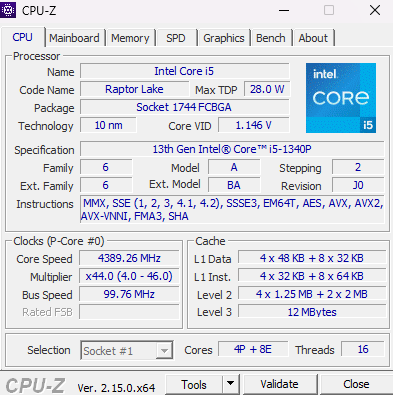
\includegraphics[width=0.8\textwidth]{Khánh/8.png}
    \caption{Intel Core i5 - 12 nhân - 16 luồng.}
\end{figure}

\subsubsection{Cache}
\begin{figure}[H]
    \centering
    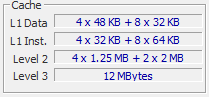
\includegraphics[width=0.8\textwidth]{Khánh/9.png}
    \caption{Hệ thống cache của máy tính bao gồm các cấp L1, L2, và L3}
\end{figure}

\subsubsection{RAM}
\begin{figure}[H]
    \centering
    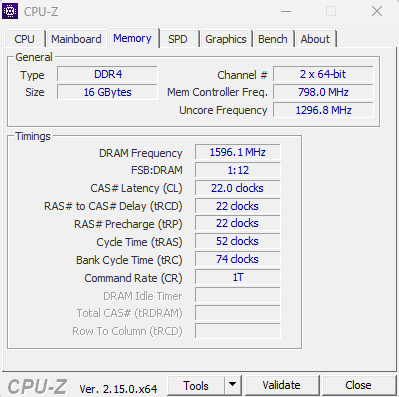
\includegraphics[width=0.7\textwidth]{Khánh/10.png}
    \caption{16Gb.}
\end{figure}


\subsubsection{Bộ nhớ ngoài}
\begin{figure}[H]
    \centering
    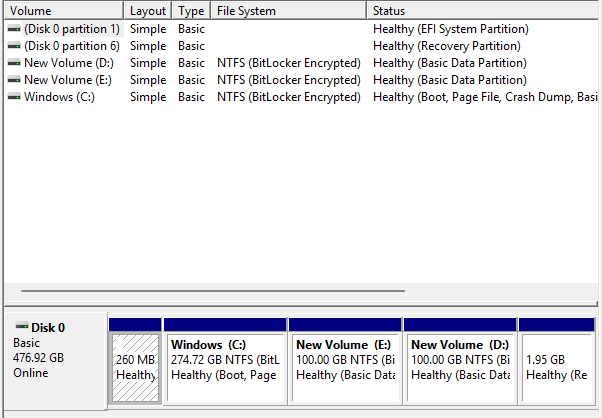
\includegraphics[width=0.8\textwidth]{Khánh/11.png}
\end{figure}


\subsubsection{Các thiết bị vào ra}
\begin{figure}[H]
    \centering
    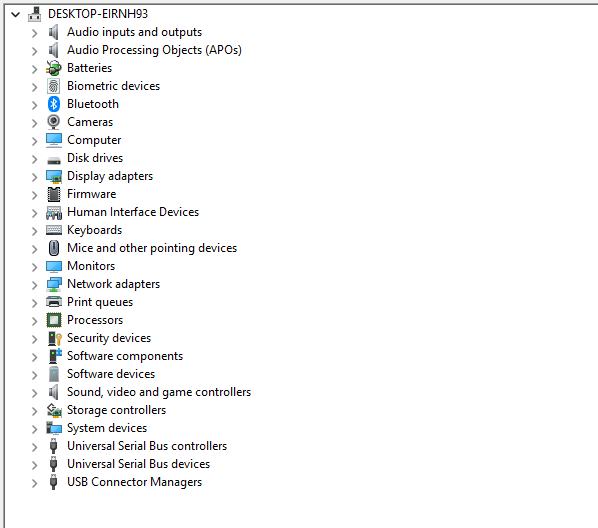
\includegraphics[width=0.8\textwidth]{Khánh/12.png}
    \caption{Bao gồm bàn phím, chuột, màn hình, và các cổng kết nối.}
\end{figure}


\subsection{Khảo sát nội dung các thanh ghi}


\subsubsection{Giải thích nội dung các thanh ghi}
Dùng công cụ Debug khảo sát nội dung các thanh ghi IP, DS, ES, SS, CS, BP, SP

\begin{itemize}
    \item Công cụ sử dụng: emu8086 microprocessor emulator
    \item Các bước thực hiện:
    \item Mở file .asm bằng phần mềm trên
    \item Chọn emulate trên thanh công cụ rồi chọn nút debug nằm cuối của cửa sổ vừa mở ra
    \item Chạy Single step để xem kết quả debug từng mã lệnh từ đầu đến cuối
\end{itemize}

\begin{figure}[H]
    \centering
    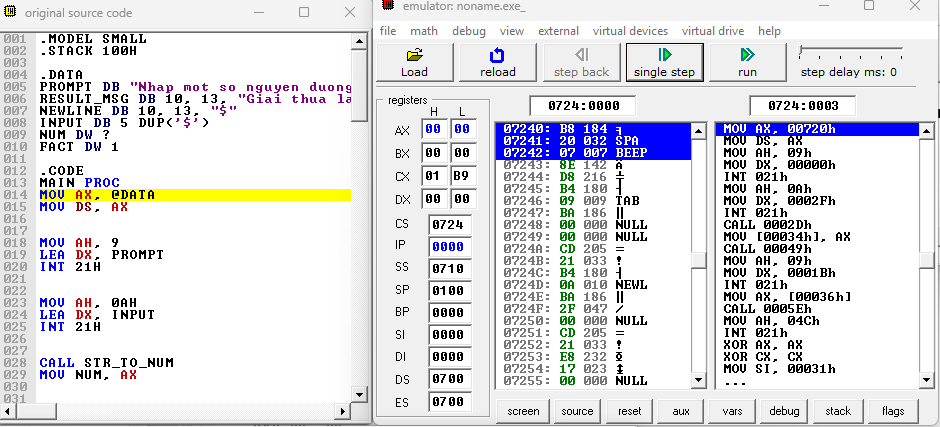
\includegraphics[width=1\textwidth]{Khánh/13.png}
\end{figure}

\begin{figure}[H]
    \centering
    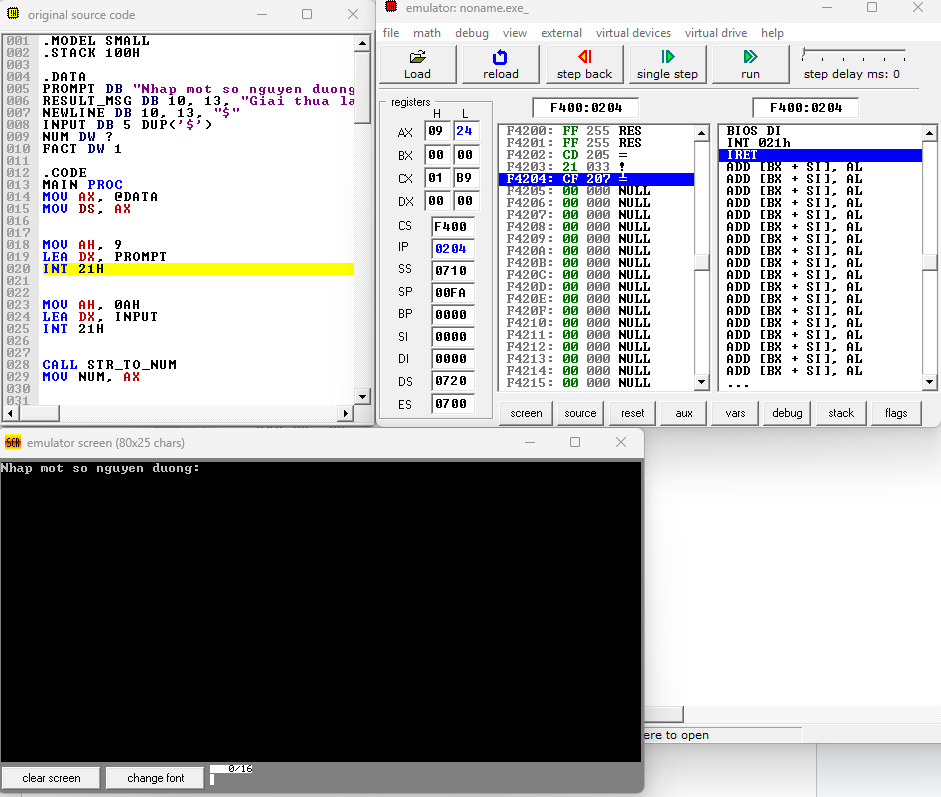
\includegraphics[width=1\textwidth]{Khánh/14.png}
\end{figure}

\begin{figure}[H]
    \centering
    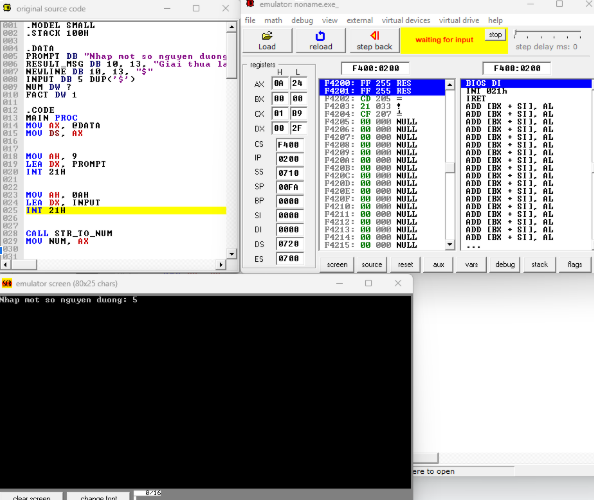
\includegraphics[width=0.85\textwidth]{Khánh/15.png}
\end{figure}

\begin{figure}[H]
    \centering
    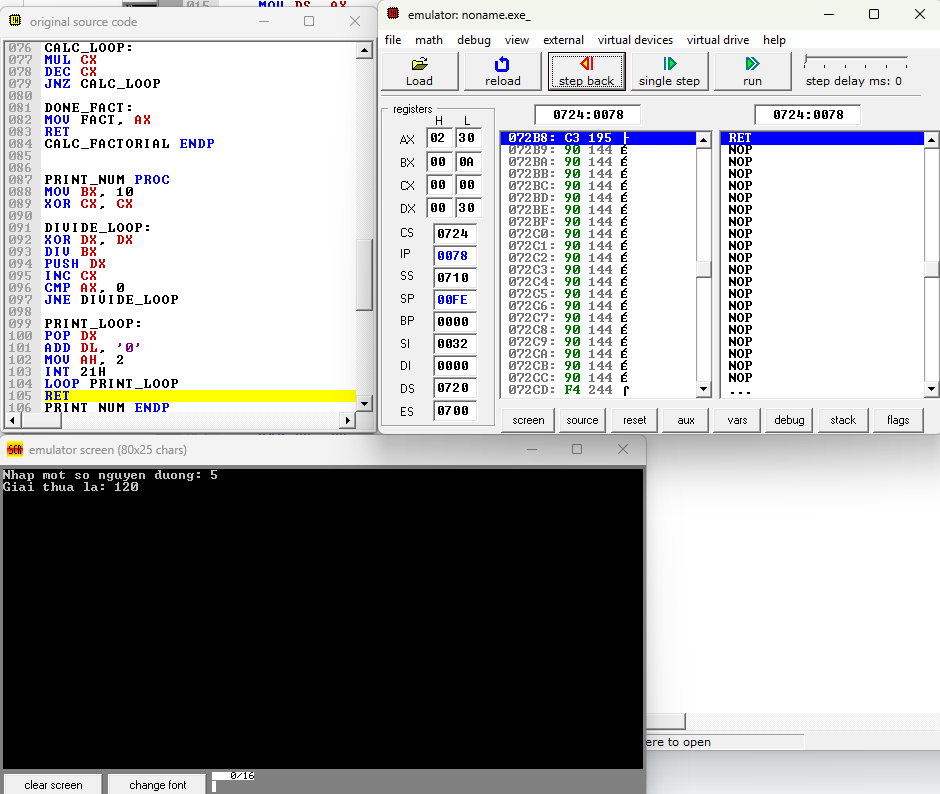
\includegraphics[width=0.85\textwidth]{Khánh/16.png}
\end{figure}


\subsection{Giải thích nội dung các thanh ghi}
Khi chương trình bắt đầu chạy, hệ điều hành tự động khởi tạo các thanh ghi, vùng nhớ và cấp phát không gian địa chỉ cho chương trình. Tương ứng với các câu lệnh trong mã nguồn, nội dung các thanh ghi có thể thay đổi hoặc không.

\subsubsection{IP (Instruction Pointer)}
\begin{itemize}
    \item IP là thanh ghi trỏ đến địa chỉ của lệnh tiếp theo sẽ được thực thi trong mã máy.
    \item Khi một chương trình được thực thi, IP được cập nhật để trỏ đến lệnh tiếp theo trong mã nguồn. Điều này giúp CPU biết lệnh nào sẽ được thực thi tiếp theo.
\end{itemize}

\subsubsection{DS (Data Segment) và SI (Source Index)}
\begin{itemize}
    \item DS là thanh ghi chỉ đến phân đoạn dữ liệu, nơi dữ liệu chương trình được lưu trữ.
    \item SI thường được sử dụng trong các phép toán dữ liệu và là một trong các thanh ghi chỉ địa chỉ.
    \item Khi chương trình yêu cầu truy cập dữ liệu từ bộ nhớ, DS và SI thường được sử dụng để xác định vị trí của dữ liệu trong bộ nhớ.
\end{itemize}

\subsubsection{SS (Stack Segment) và BP (Base Pointer)}
\begin{itemize}
    \item SS là thanh ghi chỉ đến phân đoạn ngăn xếp (stack segment), nơi các giá trị cục bộ và địa chỉ của các hàm được lưu trữ.
    \item BP thường được sử dụng để trỏ đến địa chỉ cơ sở của ngăn xếp (base of stack).
    \item Ngăn xếp được sử dụng để lưu trữ các giá trị trung gian và địa chỉ trả về từ các hàm con (subroutines) trong quá trình thực thi chương trình.
\end{itemize}

\subsubsection{SP (Stack Pointer)}
\begin{itemize}
    \item SP là thanh ghi chỉ đến đỉnh của ngăn xếp (top of stack).
    \item Khi dữ liệu được đẩy (push) hoặc rút (pop) ra khỏi ngăn xếp, SP sẽ thay đổi để chỉ đến vị trí mới nhất trong ngăn xếp.
    \item SP cũng được sử dụng để cấp phát không gian mới cho dữ liệu trong ngăn xếp.
\end{itemize}

\subsection{Cơ chế quản lý bộ nhớ}

Cụ thể, trong trường hợp của đoạn chương trình chuyển xâu ký tự thành xâu in hoa và in thường tương ứng, ta có cơ chế quản lý bộ nhớ như sau:

\subsubsection{Khởi tạo bộ nhớ}
\begin{itemize}
    \item Khi chương trình bắt đầu, HĐH sẽ cấp phát các đoạn mã (code), dữ liệu (data), và ngăn xếp (stack) cho chương trình.
    \item Đoạn mã chứa các lệnh chương trình, đoạn dữ liệu chứa các biến, và đoạn ngăn xếp dùng để lưu trữ dữ liệu tạm thời.
\end{itemize}

\subsubsection{Phân đoạn bộ nhớ}
\begin{itemize}
    \item CS (Code Segment) trỏ tới đoạn mã của chương trình.
    \item DS (Data Segment) trỏ tới đoạn dữ liệu của chương trình.
    \item SS (Stack Segment) trỏ tới đoạn ngăn xếp của chương trình.
\end{itemize}

\subsubsection{Quản lý ngăn xếp}
\begin{itemize}
    \item Ngăn xếp được sử dụng để lưu trữ tạm thời dữ liệu và địa chỉ trả về khi gọi hàm.
    \item SP được khởi tạo với giá trị từ khai báo .Stack 100H, nghĩa là kích thước ngăn xếp là 256 byte.
\end{itemize}